\chapter{Result}
For multi-label text classification there are some few models that can be used properly. In our dataset, we have eleven different classes to classify. So for our classification task, we tried three traditional classification models. They are:\\

\begin{enumerate}
    \item Multinomial Naive Bayes
    \item Logistic Regression
    \item Linear Support Vector Machine
\end{enumerate}

As mentioned earlier, we have eleven different classes they are: Black Box, Green Box, Blue Box, Yellow Box, Cyan Box, Green circle, Yellow Circle, Blue Circle, Green Triangle, Yellow Triangle and Blue Triangle. We measure accuracy of our classification using basic accuracy measurement. The comparative accuracy of classification of above mentioned model are as follow:\\

\begin{table}[h]
    \centering
    \begin{tabular}{|l|l|l|l|}
        \hline
        \multicolumn{1}{|c|}{Instruction\textbackslash{}Model} & \multicolumn{1}{c|}{Multinomial NB} & \multicolumn{1}{c|}{Linear Regression} & \multicolumn{1}{c|}{Linear SVC} \\ \hline
        Go near Black Box                                         & 1.00                                & 1.00                                   & 1.00                            \\ \hline
        Go to Green Box                                         & 0.71                                & 0.83                                   & 0.88                            \\ \hline
        Go to Blue Box                                          & 0.73                                & 0.73                                   & 0.78                            \\ \hline
        Go to Yellow Box                                        & 0.76                                & 0.73                                   & 0.78                            \\ \hline
        Go near Cyan Box                                          & 0.95                                & 1.00                                   & 1.00                            \\ \hline
        Go to Green Circle                                      & 0.56                                & 0.71                                   & 0.68                            \\ \hline
        Go to Yellow Circle                                     & 0.71                                & 0.71                                   & 0.71                            \\ \hline
        Go near Blue Circle                                       & 0.59                                & 0.83                                   & 0.83                            \\ \hline
        Go to Green Triangle                                    & 0.71                                & 0.76                                   & 0.78                            \\ \hline
        Go near Yellow Triangle                                   & 0.63                                & 0.68                                   & 0.71                            \\ \hline
        Go to Blue Triangle                                     & 0.66                                & 0.78                                   & 0.83                            \\ \hline
    \end{tabular}
    \caption{Accuracy Comparison Between Various Models}
\end{table}

So from the above table we can easily see that Linear Support Vector Classifier give us much more accuracy than any other models.\\
\newpage
A bar plot visualization of accuracy among various models is given below:


\begin{figure}[ht]
    \centering
    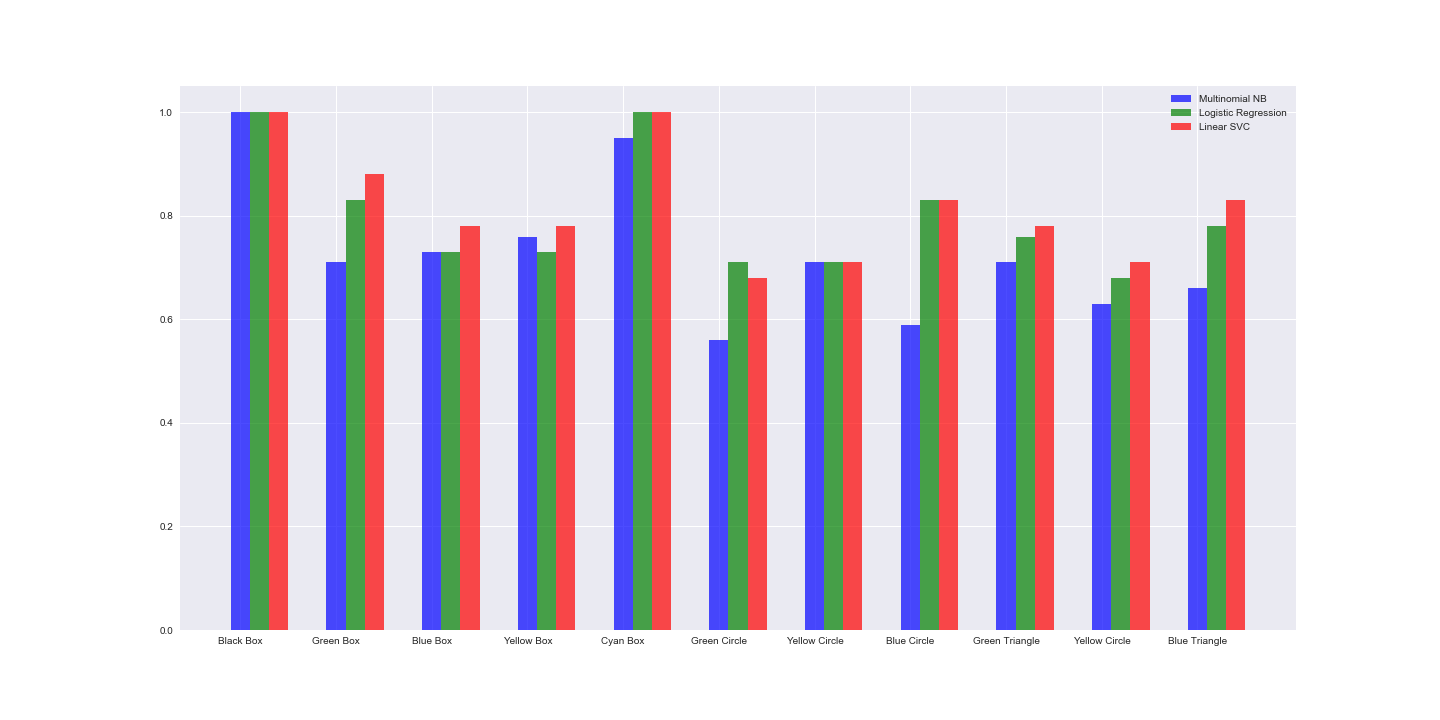
\includegraphics[scale=0.35]{visualization}
    \caption{Accuracy among different models}
\end{figure}
\vline




We still didn't try some other models and some other hyper-parameter for Linear SVC.
\newpage
	
	
